\acresetall
Learning and memory define who we are and shape who we will become.
Memory allows us to adapt to the world.
Memory and it's various components -- learning, adaptation, plasticity, association, conditioning -- are fundamental features of nervous systems across all organisms.
Over time, our understanding of memory has evolved from the earliest psychology experiments on the nature of memory \citep{Ebbinghaus1885} to a molecular understanding of the changes within the brain that occur following learning \citep{Kandel2001}.

The \ac{HPC} has been central to our study of memory at least since Scoville and Milner first reported in the 1950's on Henry Molaison (patient H.M.) who had profound anterograde amnesia following the bilateral removal of large portions of the medial temporal lobes, which includes the \ac{HPC} and parahippocampal structures \citep{Scoville1957}.
Since then, numerous studies have shown that the \ac{HPC} is essential for normal formation and recall of long term episodic and semantic memory \citep[reviewd in][]{Eichenbaum2000, Burgess2002}.

In the following sections I aim to describe an understanding of memory, the brain structures underlying it, and cellular phsyiological correlates of learning relevant to my later studies.
In discussing learning memory, I will first focus on spatial memory as a core component of episodic memory (\ref{sec:intro:hpc:memory}) and how we experimentally study it.
While learning-related changes are fundamental to every neuron in the nervous system, I will primarily focus on the role of the \ac{HPC} in learning and memory, as the \ac{HPC} is most relevant to the memory systems I will be studying (\ref{sec:intro:hpc:structure}).
Finally, I will discuss our current understanding of cellular and circuit mechanisms by which the the brain encodes and recalls memory, with a specific emphasis on hippocampal place cells underlying spatial memory (\ref{sec:intro:hpc:physiology}).

\section{Learning and Memory}






Episodic memory is 
Episodic memory \citep{Tulving1972}
% Ebbinghaus H (1885). Über das Gedachtnis, Dunker & Humbolt.
% https://books.google.com/books?id=kfA0AAAAMAAJ&ots=hjMhksDE3X&dq=Ebbinghaus%20H%20(1885).%20%C3%9Cber%20das%20Gedachtnis%2C&lr&pg=PA1#v=onepage&q&f=false

% \begin{quote}
% Episodic memory retrieves and stores information about temporally dated episodes or events, and temporal-spatial relations among these events. A perceptual event can be stored in the episodic system solely in terms of its perceptible properties or attributes, and it is always stored in terms of its autobiographical reference to the already existing contents of the episodic memory store. The act of retrieval of information from the episodic memory store, in addition to making the retrieved contents accessible to inspection, also serves as a special type input into episodic memory and thus changes the contents of the episodic memory store. The system is probably quite susceptible to transformation and loss of information. While the specific form in which perceptual input is registered into the episodic memory can at times be strongly influenced by information in semantic memory-we refer to the phenomenon as encoding-it is also possible for the episodic system to operate relatively independently of the semantic system.
% \attrib{\citealt[pgs.~385-386]{Tulving1972}}
% \end{quote}

% \begin{quote}
% Consider now a typical memory experiment in which a subject is asked to study and remember a list of familiar words or pair of words. This is an episodic memory task. The occurrence of a verbal item in a given list, at a particular time, and in specific temporal relation to other items in the list is an autobiographical episode having no necessary extra-episodic denotative reference. The subject has successfully retrieved information about this episode when he responds to the retrieval query with the reproduction if an appropriate copy of the input item.
% \attrib{\citealt{Tulving1972}}
% \end{quote}

% \begin{quote}
% Each experienced event always occurs at a particular spatial location and in a particular temporal relation to other events that already have occurred, events occurring simultaneously with it, or events that have not yet occurred. These temporal relations among experienced events are also somehow represented as properties of items in the episodic memory system. To ask a person about some item in episodic memory means to ask them when did event $E$ happen, or what events happened at time $T$. Retrieval of information of this kind from episodic memory is successful if the person can describe the perceptible properties of the event in question and more or less accurately specify its temporal relations to other events. Temporal coordinates of an event and its representation in episodic memory of course need not be specified in terms of the clock and the calendar. They could be recorded in terms of temporal occurrences of other events in some as yet little understood manner.
% \attrib{\citealt[pg.~388]{Tulving1972}}
% \end{quote}

Eichenbaum H, Yonelinas AR, Ranganath C (2007): The medial tempo- ral lobe and recognition memory. Annu Rev Neurosci 30:123–152.
Milner B, Squire LR, Kandel ER (1998): Cognitive neuroscience and the study of memory. Neuron 20:445–468.
23.
Fortin NJ, Wright SP, Eichenbaum H (2004): Recollection-like memory retrieval in rats is dependent on the hippocampus. Nature 431:188– 191.
Sauvage MM, Fortin NJ, Owens CB, Yonelinas AP, Eichenbaum H (2008): Recognition memory: Opposite effects of hippocampal dam- age on recollection and familiarity. Nat Neurosci 11:16–18.

\subsection{Spatial memory}\label{sec:intro:hpc:spatial}
Studied because it is tractable.
We have good behavioral tests in rodents.
We found cells that appear to encode the memory itself.
Allocentric navigation in particular is \ac{HPC}-dependent \citep{OKeefe1978, Smith1989}, not egocentric.

\subsubsection{Spatial memory is a core component of episodic memory}\label{sec:intro:hpc:spatial-episodic}
In 1972 Endel Tulving coined the term \textsc{episodic memory}, describing it as follows:

\begin{quote}
Episodic memory retrieves and stores information about temporally dated episodes or events, and temporal-spatial relations among these events...Each experienced event always occurs at a particular spatial location and in a particular temporal relation to other events that already have occurred, events occurring simultaneously with it, or events that have not yet occurred.
\attrib{\citealt{Tulving1972}}
\end{quote}

As this interpretation suggests, the specific of the events itself are inseparable from the time at which it occurred and the location of the event (or individual aspects of the event).
This is most obvious in autobiographical episodic memory, where experiences (e.g. waiting in line to get lunch) are remembered along with the location (e.g. Mike's Bagels at 168th and Broadway) and the time (e.g. last Tuesday around 2PM) they occurred.
This applies to psychological memory tests as well, such as remembering words on a list, where the temporal order of items on the list (I saw `orange' before `banana') and the visio-spatial arrangement of the words on the paper list (`boat' was written above `car') are core components of the stored memory.
While certain aspects of episodic memory are clearly organized separately in the brain (e.g. fearful associations in the amygdala) the centrality of spatial components to episodic memory causes deficits to manifest more generally as 

\section{Spatial memory and navigation}
Spatial memory is fundamental to our daily lives; it allows us to know where we are, where we have been, and how to get to where we want to go.
The core of the mammalian spatial navigation system is found in the hippocampal formation in the medial temporal lobe.
Spatial navigation consists of two primary components: location relative to an allocentric map of the world, and egocentric update cues arising from orientation (\textsc{head direction cells}) and other vestibular input.

Throughout the \ac{HPC} (dentate gyrus, CA3, CA2, and CA1) there are principal cells that fire at specific locations within an environment (\textsc{place cells}).
Within the entorhinal coretx, principal cells take on a variety of spatial firing properties, but one of the main categories are cells that fire at regularly spaced intervals throughout an environment (`grid cells').
Place cells and grid cells together form the cellular foundation for the mammalian navigation system, and their discovery was recently awarded with the Nobel Prize in Medicine.


\subsection{Place cells}
Pyramidal cells in hippocampal area CA1 are the principal excitatory neuron in that region and the primary output from the \ac{HPC}.
As an animal explores an environment these pyramidal cells show sparse spatially-modulated changes in firing rates (place cells) that are established rapidly and subsequently remain stable \citep{O'Keefe1971}\citep{Frank2004}.
These place cells form an allocentric map of the environment, which is essential for normal episodic memory function \citep{Smith2006c}\citep{Nakazawa2004}\citep{Buzsaki2013}.

\section{Remapping}
Place cells, like other forms of memory, are constantly trying to balance two competing constraints: on the one hand, their firing needs to be stable in order to be a helpful representation of the environment, but on the other hand, their firing needs to be plastic enough to constantly encode new environments, forget irrelevant information, and adapt to new features.
Place cells changing their firing properties to incorporate new features of the world is known as \textsc{remapping}.
A given place cell is defined by it's spatial tuning -- it's place field -- and it's firing rate gain with the place field.
These seem to be independent factors, as either can remap separately.
\textsc{Global remapping} is the collective remapping of place field locations across a population of place cells.
Alternatively, \textsc{rate remapping} is a change in place field gain (the ratio of firing rate in to out of the place field), while place fields locations remain fixed.
While place field location and firing rate gain remap separately....\textsc{partial remapping}.



\section{Spatial reward learning}\label{sec:intro:hpc:spatial-reward}
Tests of spatial memory are fundamental tools for rodent researchers.
The most widely used assay of spatial memory is the \textsc{Morris water maze} \citep{Morris1984}.
While there is variability in the details of the protocol, the general structure is usually the same.
Briefly, the `maze' is a large water-filled tub with a single hidden platform under the surface of the water.
Mice or rats are placed in the maze and over successive trials eventually learn to use distal cues around the room to locate the platform.
Probe trials generally consist of removing the platform and scoring the fraction of time spent in the correct quadrant as a measure of spatial memory.
More recently, virtual reality variations of the Morris water maze have been developed that allow for head-fixed spatial learning tasks in rodents \citep{Aronov2014} or the ability to mirror rodent experimental paradigms in humans \citep{}. 

Conceptually similar, but drier, are the Barnes or cheeseboard maze \citep{Barnes1979}\citep{Kesner1991}\citep{Dupret2010a}.
These mazes are consist of a large platform with holes throughout.
These holes can either be escapes for the mice/rats to avoid the exposure of the platform, or baited/rewarded.
Either way, degree of learning can be quantified by latency to finding the correct location or time spent near previously rewarded locations during un-rewarded probe trials.



\section{Structure}\label{sec:intro:hpc:structure}
The hippocampal-formation is one of the best characterized neuronal circuits within the mammalian brain.
Primary excitatory projections neurons transfer information from the subiculum to the entorhinal cortex to the hippocampus-proper.
The principal neurons in the \ac{HPC} communicate through the classically-defined trisynaptic loop: perforant path fibers project from the entorhinal cortex (EC) to granule cells in the dentate gyrus, which in turn send mossy fiber projections to CA3 that finally travel along the Schaffer collateral pathway and synapse upon proximal apical and basal dendrites of CA1 pyramidal cells (CA1PCs).
CA1PCs then send processed information to cortical and subcortical areas, including return projections back to deep layers of EC.
In addition, distal dendrites of CA1PCs receive direct projections from EC along the temporammonic pathway and CA1PC activity is also directly regulated by a diverse population of local GABAergic interneurons.
Finally, both principal neurons and GABAergic interneurons are targeted by afferents from neuromodulatory nuclei, including cholinergic and GABAergic projections from the medial septum  \citep{Klausberger2008}, serotonergic and glutamatergic projections from the raphe nuclei \citep{Varga2009}, as well as dopaminergic and noradrenergic projections from the ventral tegmental area \citep{Gasbarri1997} and locus coeruleus \citep{Foote1983}.


Burwell RD (2000): The parahippocampal region: Corticocortical connectivity. Ann N Y Acad Sci 911:25–42.
\subsection{CA1}
\begin{figure}
	\centering
	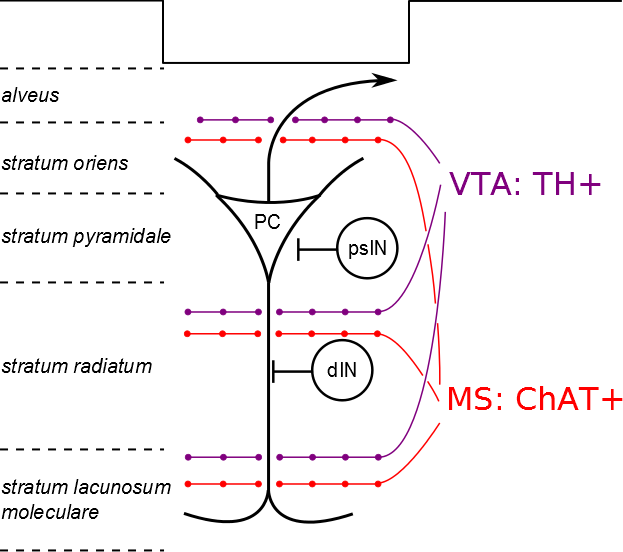
\includegraphics[width=0.5\textwidth]{intro/CA1-schematic_INs_VTA_MS}
	\caption{Schematic of major inputs to CA1 pyramidal cells}
	\label{fig:intro:hpc:CA1_schematic}
\end{figure}

\section{Neurons and Memory}\label{sec:intro:hpc:physiology}


\subsection{Other}
In discussing the role of the \ac{HPC}, I've focused on spatial memory, but this is clearly not the sole role of the \ac{HPC}.
Social
Time
conversion to longterm memory
environment
pattern completion/separation

